\section{Introduction}
Several signs like speed limit number, speed limit end, pedestrian island and turn signs are single contour. Detection of these signs are somewhat simpler compared to\hyperref[chap:MultiContour]{ multi contour signs}.

\section{Detection process}
\begin{figure}[h]
    \centering
    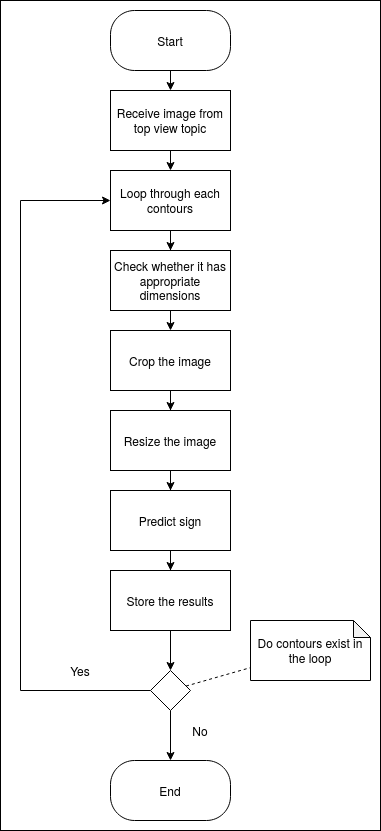
\includegraphics[scale=0.40]{images/SIngleContourFlowDiagram.png}
    \caption{Flow chart of detection of single contour sign}
    \label{fig:SingleContourDetectionFlowChart}
\end{figure}

\subsection{Receive image from top view topic}
\label{subsec:RecieveImageFromTopView}
The code in \emph{DetectSignsOnLane::init()} function registers to topic which has top view of the lane.

\subsection{Loop through each contours}
\label{subsec:LoopThroughContours}
The code in \emph{DetectSignsOnLane::detectSignsFromRawImage()} function loops through the contours of the image in search of the lane signs.

\subsection{Check whether it has appropriate dimensions}
Each contour is checked for their dimensions in different functions based on the sign we are looking for and also each sign has different dimensions. The functions in which dimensions of contour is checked and the constants of dimensions on which they are checked against are mentioned below.
\begin{table}[h!]
\centering
\begin{tabular}{|c|c|}
\hline
    Sign Type & Function name\\
\hline
    Number &  \small{\emph{DetectSignsOnLane::isContourANumber()}}\\
    Turn left/right &  \small{\emph{DetectSignsOnLane::isContourATurnSign()}}\\
    End of speed limit &  \small{\emph{DetectSignsOnLane::isContourASpeedEnd()}}\\
    Pedestrian island &  \small{\emph{DetectSignsOnLane::isContourAPedestrianIsland()}}\\
\hline
\end{tabular}
\caption{Different functions where different signs are checked}
\end{table}
    
\begin{table}[h!]
\centering
\begin{tabular}{|c|c|}
\hline
    Sign Type & Constants on which contours are checked against\\
\hline
    Number & \vtop{\hbox{\strut \scriptsize{NUMBER\_SIGN\_RECT\_MIN\_WIDTH, \,NUMBER\_SIGN\_RECT\_MAX\_WIDTH}}\hbox{\strut \scriptsize{NUMBER\_SIGN\_RECT\_MIN\_HEIGHT, \,NUMBER\_SIGN\_RECT\_MAX\_HEIGHT}}}\\
    \hline
    Turn left/right & \vtop{\hbox{\strut \scriptsize{ARROW\_SIGN\_RECT\_MIN\_WIDTH, \,ARROW\_SIGN\_RECT\_MAX\_WIDTH}}\hbox{\strut \scriptsize{ARROW\_SIGN\_RECT\_MIN\_HEIGHT, \,ARROW\_SIGN\_RECT\_MAX\_HEIGHT}}}\\
    \hline
    End of speed limit & \vtop{\hbox{\strut \scriptsize{SPEEDEND\_SIGN\_RECT\_MIN\_WIDTH, \,SPEEDEND\_SIGN\_RECT\_MAX\_WIDTH}}\hbox{\strut \scriptsize{SPEEDEND\_SIGN\_RECT\_MIN\_HEIGHT, \,SPEEDEND\_SIGN\_RECT\_MAX\_HEIGHT}}}\\
    \hline
    Pedestrian island & \vtop{\hbox{\strut \scriptsize{PEDESTRIAN\_ISLAND\_MIN\_WIDTH, \,PEDESTRIAN\_ISLAND\_MAX\_WIDTH}}\hbox{\strut \scriptsize{PEDESTRIAN\_ISLAND\_MIN\_HEIGHT, \,PEDESTRIAN\_ISLAND\_MAX\_HEIGHT}}}\\
\hline
\end{tabular}
\caption{Constraints on dimensions of different signs}
\label{table:SingleContourDimensionConstraint}
\end{table}

\subsection{Crop the image}
The contours which happens to have appropriate dimensions of any of the single contour sign, then image will be cropped up to the contour. This step is done in \emph{DetectSignsOnLane::cropAndCompress} \newline \emph{Image()} function.
\begin{figure}[h!]
\begin{subfigure}{0.5\textwidth}
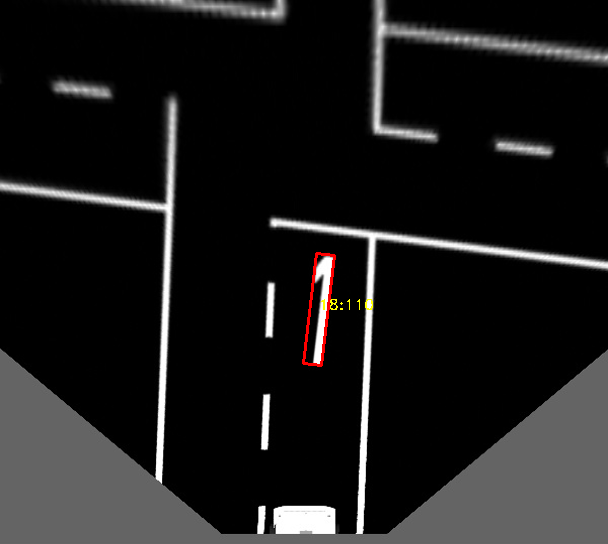
\includegraphics[scale=0.5]{images/BeforeCropping.png} 
\caption{Before cropping}
\end{subfigure}
\begin{subfigure}{0.5\textwidth}
\centering

\includegraphics[scale=2.5]{images/AfterCropping.png} 
\caption{After cropping}
\end{subfigure}
\caption{Before and after cropping the image for single contour sign}
\label{fig:BeforeAfterCropSingleContour}
\end{figure}

\subsection{Resize the image}
The image which is cropped will be resized to 20x20 pixel size image. This step and previous steps are preprocessing before asking the model to predict the sign.
\begin{figure}[h!]
\begin{subfigure}{0.5\textwidth}
\centering

\includegraphics[scale=1]{images/AfterCropping.png} 
\caption{Before resizing}
\end{subfigure}
\begin{subfigure}{0.5\textwidth}
\vspace{2.2cm}
\centering

\includegraphics[scale=1]{images/AfterResizing.png} 
\caption{After resizing}
\end{subfigure}
\caption{Before and after resizing the image for single contour sign}
\label{fig:BeforeAfterResizeSingleContour}
\end{figure}

\subsection{Predict sign}
\label{sec:PredictSign}
After above preprocessing step, the 20x20 pixel will be sent to the model. The model will predict the sign by outputting a number. \emph{DetectSignsOnLane::predictSign()} is the function that predicts the sign and outputs the number. Details about how to train a model is discussed in upcoming \autoref{chap:TrainingClassifier}. The following is the table that describes the meaning of each number predicted by the model.
\begin{table}[h!]
\centering
\begin{tabular}{|c|c|}
\hline
    Number from model & Sign Type\\
    \hline
    0 & Number sign 0\\
    1 & Number sign 1\\
    2 & Number sign 2\\
    3 & Number sign 3\\
    4 & Number sign 4\\
    5 & Number sign 5\\
    6 & Number sign 6\\
    7 & Number sign 7\\
    8 & Number sign 8\\
    9 & Number sign 9\\
    10 & Speed limit ends\\
    11 & Turn left\\
    12 & Turn right\\
    13 & False detections\\
    14 & Inverted numbers\\
    15 & Pedestrian island\\
\hline
\end{tabular}
\caption{Different sign and their associated number}
\label{table:NumberFromModel}
\end{table}

\subsection{Store the results}
\label{sec:SingleContStoreResults}
All the signs that are detected in a single image are stored in a list and the results are published. Details of the publishing the results are discussed in \autoref{chap:PublishResults}.